\subsection{Упражнение 1}

При взятии выборок из сигнала при слишком низкой чистоте кадров составляющие, большие частоты заворота дадут биения. В таком случаее эти компоненты не отфильтруешь, посколько они неотличимы от более низких частот. Полезно отфильтровать эти частоты до выборки: фильтр НЧ, используемый для этой цели, называется фильтром сглаживания. Вернитесь к примеру "Соло на барабане", примените фильтр НЧ до выборки, а затем, опять с помощью фильтра НЧ, удалите спектральные копии, вызванные выборкой. Результат должен быть идентицент отфильтрованному сигналу.

\begin{lstlisting}[language=Python]
if not os.path.exists('263868__kevcio__amen-break-a-160-bpm.wav'):
    !wget https://github.com/AllenDowney/ThinkDSP/raw/master/code/263868__kevcio__amen-break-a-160-bpm.wav
    
wave = read_wave('263868__kevcio__amen-break-a-160-bpm.wav')
wave.plot()
\end{lstlisting}
\begin{figure}[H]
	\begin{center}
		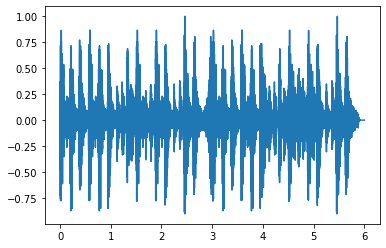
\includegraphics[scale=1]{fig/lab11/lab11_5_0.png}
		\caption{График "Соло на барабане"}
	\end{center}
\end{figure}

\begin{lstlisting}[language=Python]
spectrum = wave.make_spectrum(full=True)
spectrum.plot()
\end{lstlisting}
\begin{figure}[H]
	\begin{center}
		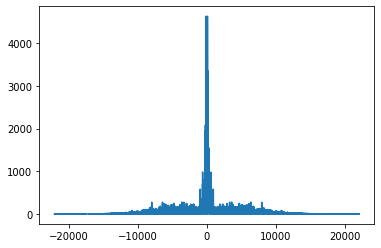
\includegraphics[scale=1]{fig/lab11/lab11_8_0.png}
		\caption{Спектр сигнала}
	\end{center}
\end{figure}

Фильтр низких частот:

\begin{lstlisting}[language=Python]
factor = 3
framerate = wave.framerate / factor
cutoff = framerate / 2 - 1

spectrum.low_pass(cutoff)
spectrum.plot()
\end{lstlisting}
\begin{figure}[H]
	\begin{center}
		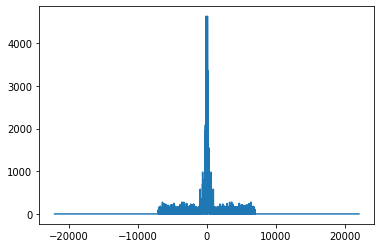
\includegraphics[scale=1]{fig/lab11/lab11_11_0.png}
		\caption{Отфильтрованный сигнал}
	\end{center}
\end{figure}

Функция сэмплирования:

\begin{lstlisting}[language=Python]
def sample(wave, factor):
    """Simulates sampling of a wave.
    
    wave: Wave object
    factor: ratio of the new framerate to the original
    """
    ys = np.zeros(len(wave))
    ys[::factor] = wave.ys[::factor]
    return Wave(ys, framerate=wave.framerate) 
\end{lstlisting}



\begin{lstlisting}[language=Python]
sampled_spectrum = sampled.make_spectrum(full=True)
sampled_spectrum.plot()
\end{lstlisting}
\begin{figure}[H]
	\begin{center}
		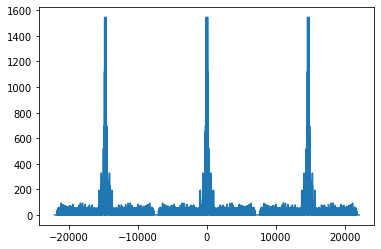
\includegraphics[scale=1]{fig/lab11/lab11_16_0.png}
		\caption{Получившийся спектр}
	\end{center}
\end{figure}

Избавляемся от спектральных копий:
\begin{lstlisting}[language=Python]
sampled_spectrum.low_pass(cutoff)
sampled_spectrum.plot()
\end{lstlisting}
\begin{figure}[H]
	\begin{center}
		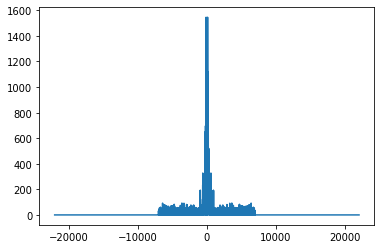
\includegraphics[scale=1]{fig/lab11/lab11_18_0.png}
		\caption{Результат избавления от копий}
	\end{center}
\end{figure}

Получившийся звук отличается, чтобы понять в чём проблема сравним спектры:

\begin{lstlisting}[language=Python]
spectrum.plot()
sampled_spectrum.plot()
\end{lstlisting}
\begin{figure}[H]
	\begin{center}
		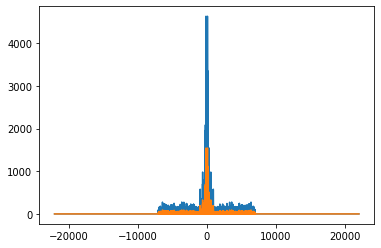
\includegraphics[scale=1]{fig/lab11/lab11_21_0.png}
		\caption{Сравнение спектров}
	\end{center}
\end{figure}

Надо увеличить ампилитуду в 3 раза:

\begin{lstlisting}[language=Python]
sampled_spectrum.scale(factor)
sampled_spectrum.plot()
spectrum.plot()
\end{lstlisting}
\begin{figure}[H]
	\begin{center}
		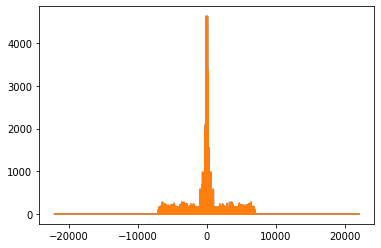
\includegraphics[scale=1]{fig/lab11/lab11_23_0.png}
		\caption{Сравнение спектров}
	\end{center}
\end{figure}

Полученный звук, действительно, не сильно отличается от исходного.

\subsection{Вывод}

В данной работе были проверены свойства выборок и прояснены биения и заворот частот.
